\documentclass[a4paper,12pt]{article} %размер бумаги устанавливаем А4, шрифт 12пунктов
\usepackage[utf8]{inputenc}
\usepackage{csquotes}
\usepackage[english,russian]{babel}%используем русский и английский языки с переносами
\usepackage{biblatex}
\bibliography{refs}
\usepackage{amssymb,amsfonts,mathtext,enumerate,float} %подключаем нужные пакеты расширений
\usepackage{textcomp}
\usepackage{adjustbox}
\usepackage{graphicx} %хотим вставлять в диплом рисунки?
\makeatletter
\makeatother
\usepackage{sagetex}
\usepackage{geometry} % Меняем поля страницы
\geometry{left=2cm}% левое поле
\geometry{right=1.5cm}% правое поле
\geometry{top=1cm}% верхнее поле
\geometry{bottom=2cm}% нижнее поле
\usepackage{amsmath} %отображение математической нотации

\usepackage{caption, subcaption} %подписи
\usepackage{tabularx} 
\usepackage{threeparttable}
\captionsetup[table]{labelsep = endash, singlelinecheck=false}


\begin{document}

\newcommand\tline[2]{$\underset{\text{#1}}{\text{\underline{\hspace{#2}}}}$}
\newcommand\nameLine[3]{$\underset{\text{#1}}{\text{\underline{\text{#2}\hspace{#3}}}}$}

\begin{titlepage}
	\centering
	{\fontsize{12pt}{5cm}\selectfont \bfseries Министерство образования и науки Российской Федерации} \\ \vspace{0.5cm}
	{\fontsize{7pt}{5cm}\selectfont ФЕДЕРАЛЬНОЕ ГОСУДАРСТВЕННОЕ АВТОНОМНОЕ ОБРАЗОВАТЕЛЬНОЕ УЧРЕЖДЕНИЕ ВЫСШЕГО ПРОФЕССИОНАЛЬНОГО ОБРАЗОВАНИЯ} \\ 
	\vspace{1cm}
	{\fontsize{12pt}{5cm}\selectfont \bfseries САНКТ-ПЕТЕРБУРГСКИЙ УНИВЕРСИТЕТ ИНФОРМАЦИОННЫХ ТЕХНОЛОГИЙ, МЕХАНИКИ И ОПТИКИ} \\ \vspace{1.5cm}
	
	{\fontsize{14pt}{5cm}\selectfont Кафедра \hspace{1cm} \underline{Систем Управления и Информатики}  \hspace{1cm} Группа \underline{Р3340}} \\
	
	\vspace{2cm}
	
	{\fontsize{20pt}{5cm}\selectfont \bfseries Лабораторная работа №9} \\
	{\fontsize{20pt}{5cm}\selectfont \bfseries “Экспериментальное построение частотных характеристик типовых динамических звеньев”} \\
	\vspace{0.2cm}
	{\fontsize{14pt}{5cm}\selectfont Вариант - 10} \\
	
	\vspace{1.5cm}
	
	\flushleft
	{Выполнилa \hspace{1.8cm} \nameLine{(фамилия, и.о.)}{Ким А. А.}{7cm} (подпись)} \\
	
	\vspace{2cm}
	
	{Проверил \hspace{2cm} \tline{(фамилия, и.о.)}{9cm} (подпись)} \\
	
	\vspace{5cm}
	
	"\underline{\hspace{0.7cm}}"\hspace{0.2cm}\underline{\hspace{2cm}}\hspace{0.2cm}20\underline{\hspace{0.7cm}}г. \hspace{2cm} Санкт-Петербург, \hspace{2cm} 20\underline{\hspace{0.7cm}}г. \\ \vspace{1cm}
	
	Работа выполнена с оценкой \hspace{1cm} \underline{\hspace{8cm}} \\ 
	\vspace{1cm}
	Дата защиты "\underline{\hspace{0.7cm}}"\hspace{0.2cm}\underline{\hspace{2cm}}\hspace{0.2cm}20\underline{\hspace{0.7cm}}г.
\end{titlepage}

\paragraph{Цель работы:}Ознакомление с экспериментальными методами построения областей устойчивости линейных динамических систем и изучение влияния на устойчивость системы её параметров.%*-без нумерации
\paragraph{Вариант задания.} Задана линейная система третьего порядка, структурная схема которой представлена на рисунке 1. Система имеет три параметра ~--- постоянные времени $T_1$,$T_2$ и коэффициент передачи $K$. При исследовании системы постоянную времени $T_1$ будем считать фиксированной и равной 2,75, а область устойчивости будем определять на плоскости двух параметров $K$ и $T_2$. Причем диапазон изменения постоянной времени $T_2$ ~--- от 0,1 до 5 с. Тип устойчивости системы будет определять по виду переходного процесса при нулевом входном воздействии $g(t)=0$ и ненулевом начальном значении выходной переменной $y(0)=1$.
\begin{figure}[h!]
	\centering
	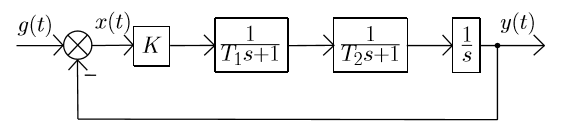
\includegraphics[width=0.8\linewidth]{scheme/scheme1.png}
	\caption{Структурная схема моделируемой линейной системы третьего порядка}
\end{figure} 

\newpage
\begin{center}
    \section{Построение границы устойчивости на плоскости двух параметров $K$ и $T_2$ методом математического моделирования}
\end{center}
\par На рисунке 2 представлена схема моделирования для системы с заданными параметрами.
\begin{figure}[h!]
	\centering
	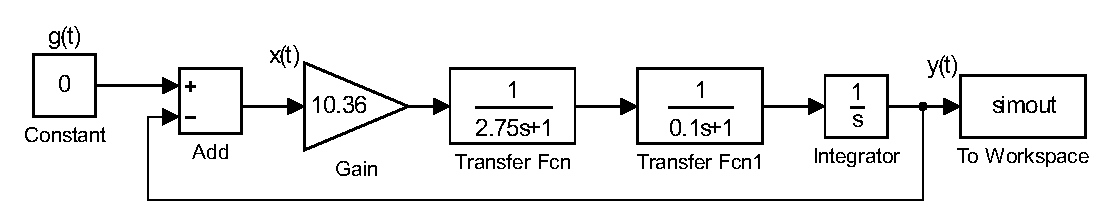
\includegraphics[width=1\linewidth]{scheme/scheme.eps}
	\caption{Структурная схема моделируемой системы}
\end{figure}
 
Будем менять значение $T_2$ и подбирать коэффициент передачи $K$ таким образом, чтобы система находилась на границе устойчивости. Данные, необходимые для построения границы устойчивости приведены в таблице 1, графическое изображение границы устойчивости ~--- на рисунке 3.
\begin{table}[h!]
		\renewcommand{\arraystretch}{1.8} %строки
		\centering
		\begin{threeparttable}
		\caption{Данные необходимые для построения границы устойчивости системы}
			\begin{tabular}{|c|c|c|c|c|c|c|c|c|c|c|}
				\hline $T_2$ & 0,1 & 0,2 & 0,3 & 0,4 & 0,5 & 0,75 & 1 & 2 & 3 & 5\\
				\hline $K$ & 10,36 & 5,36 & 3,69 & 2,86 & 2,36 & 1,69 & 1,36 & 0,86 & 0,69 & 0,56\\
				\hline
			\end{tabular}	
		\end{threeparttable}
\end{table} 
\begin{figure}[h!]
	\centering
	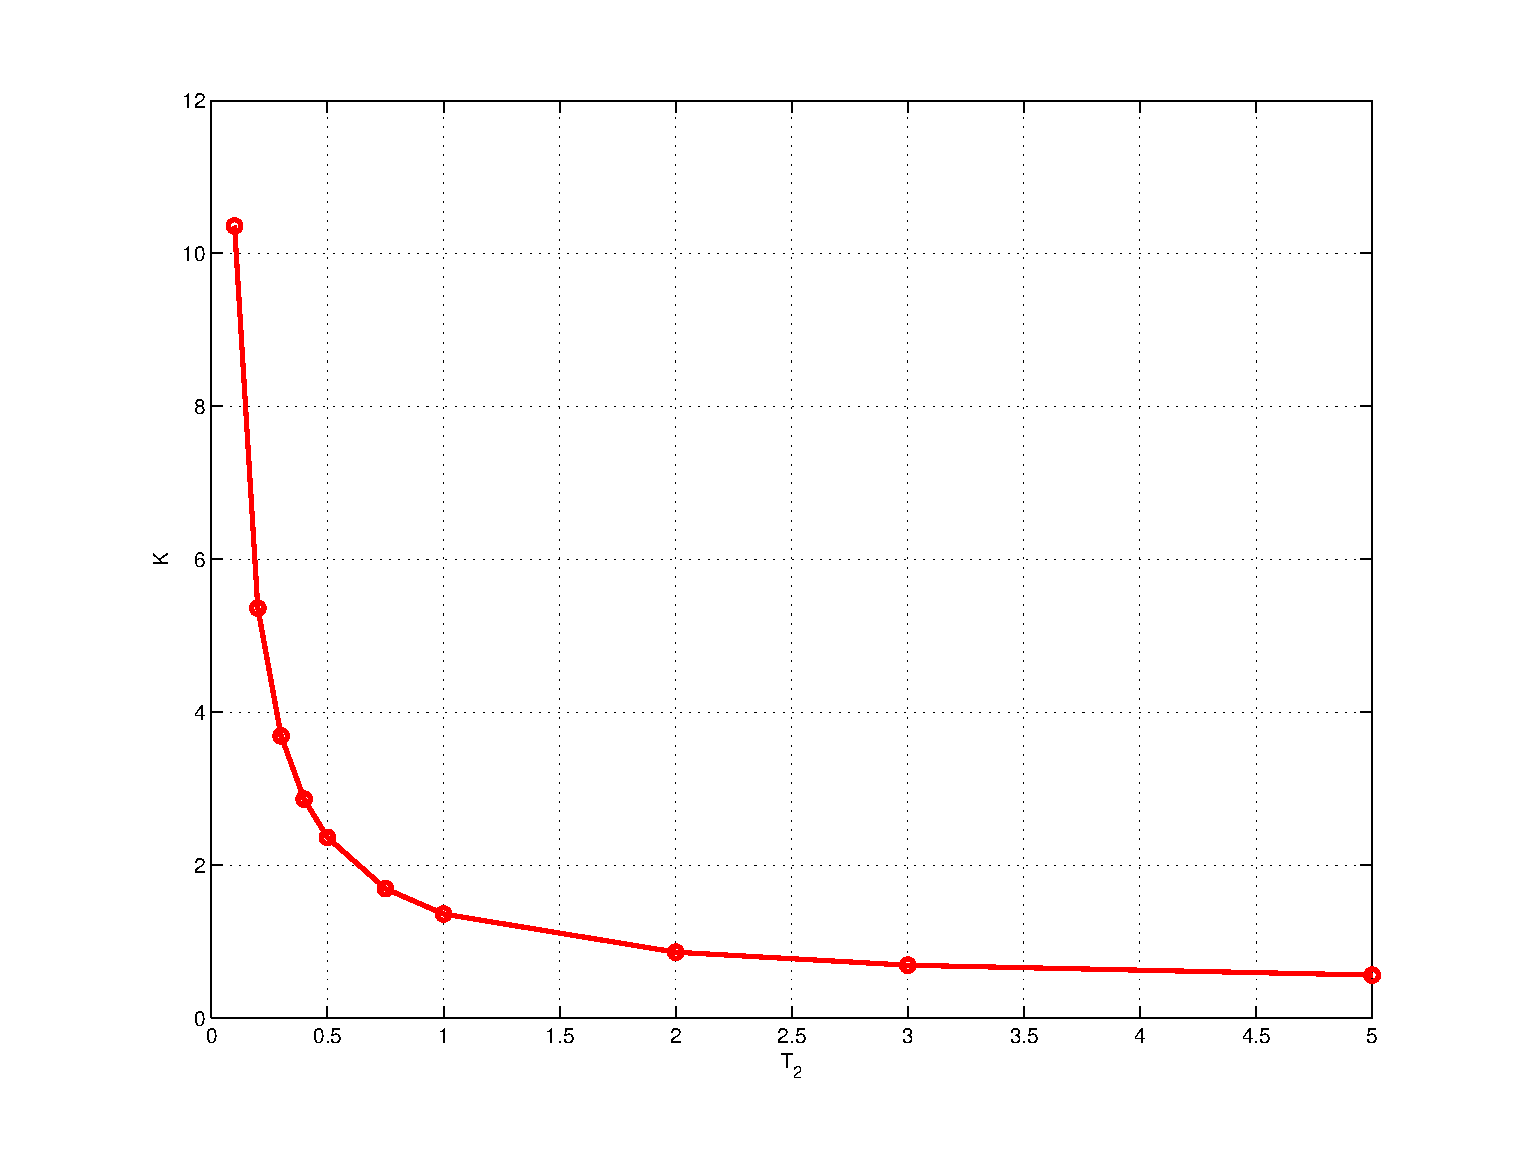
\includegraphics[width=1\linewidth]{scheme/plot0.eps}
	\caption{Граница устойчивости на плоскости двух параметров $K, T_2$, построенная методом математического моделирования}
\end{figure}

Графики переходных процессов для устойчивой системы, неустойчивой и системы, находящейся на границе устойчивости представлены соответственно на 4, 5 и 6 рисунках.
\begin{figure}[H]
	\centering
	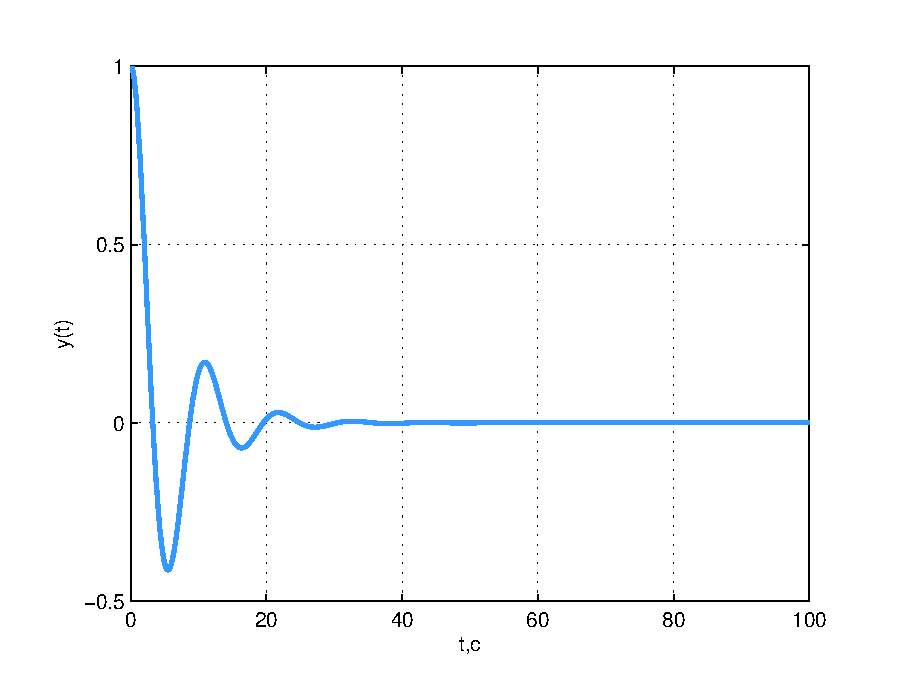
\includegraphics[width=1\linewidth]{scheme/plot1.eps}
	\caption{Система устойчива}
\end{figure}
\begin{figure}[H]
	\centering
	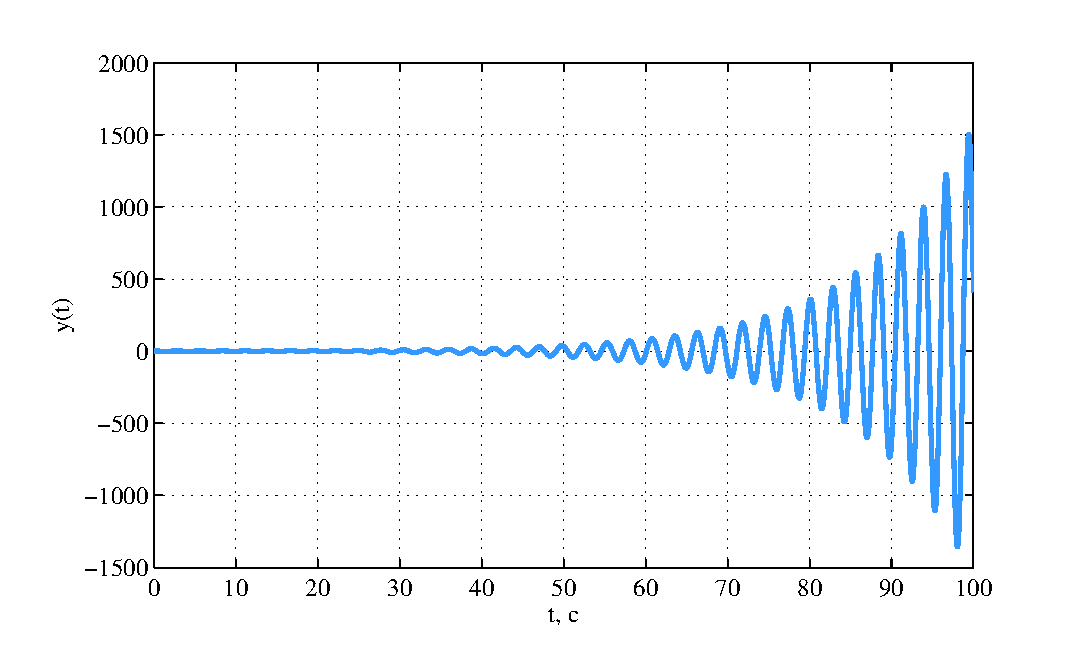
\includegraphics[width=1\linewidth]{scheme/plot2.eps}
	\caption{Неустойчивая система}
\end{figure}
\begin{figure}[H]
	\centering
	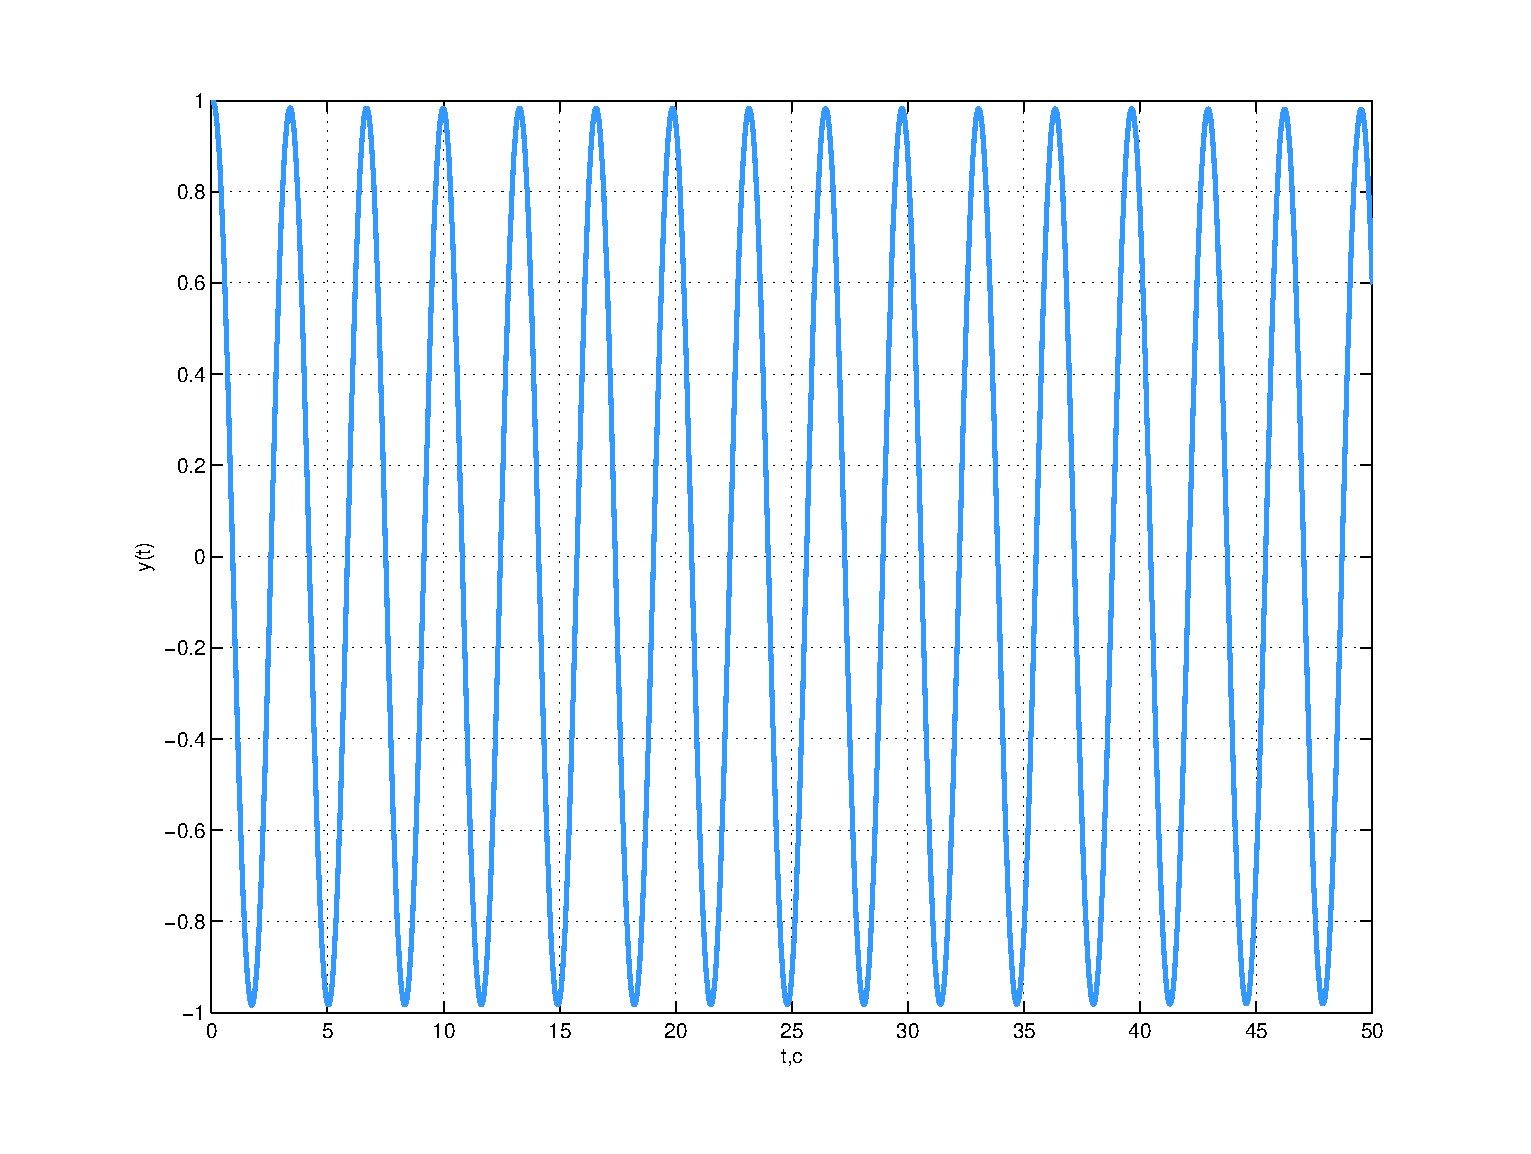
\includegraphics[width=1\linewidth]{scheme/plot3.eps}
	\caption{Система, находящаяся на границе устойчивости}
\end{figure}

\newpage
\begin{center}
    \section{Теоретический расчет границы устойчивости с использованием критерия Гурвица}
\end{center}
 
 
Передаточная функция замкнутой системы выглядит следующим образом:
\begin{equation} W(s) = \frac{\Phi(s)}{1 + \Phi(s)}, \end{equation}
где $\Phi(s)$ - передаточная функция разомкнутой системы.
\begin{equation} 
\Phi(s) = K\cdot\frac{1}{T_1s + 1}\cdot\frac{1}{T_2s + 1}\cdot\frac{1}{s} = \frac{K}{T_1T_2s^3 + (T_1 + T_2)s^2 +s},
\end{equation}
\par
Тогда \begin{equation} W(s) = \frac{K}{T_1T_2s^3 + (T_1 + T_2)s^2 +s + K}. \end{equation}
\par
На основании характеристического уравнения, построенного по передаточной функции замкнутой системы, составим матрицу Гурвица для определения границы устойчивости:
\[
\begin{vmatrix}
$$T_1 + T_2$$ & $$K$$ & 0\\
$$T_1T_2$$ & 1 & 0\\
0 & $$T_1 + T_2$$ & $$K$$
\end{vmatrix}
\]
\par
По критерию Гурвица для устойчивости системы необходимо, чтобы главные миноры матрицы были положительны. 
\begin{equation}
    \begin{cases}
        $$T_1 + T_2 > 0$$\\
        $$T_1 + T_2 - KT_1T_2 > 0$$\\
        $$K(T_1 + T_2) - K^2T_1T_2 > 0$$
    \end{cases}
\end{equation}
\par
Если минор $n - 1$ порядка равен 0, то система будет находится на колебательной границе устойчивости. По условию $T_1$ и $T_2$ больше 0, тогда для определения границы устойчивости воспользуемся выражением:
\begin{equation}
    K = \frac{T_1 + T_2}{T_1T_2} =  \frac{1}{T_1} + \frac{1}{T_2}
\end{equation}
    
Используя выражение (5), найдём $K$. Полученные значения запишем в таблицу 2.
\begin{table}[h!]
    \renewcommand{\arraystretch}{1.8} %строки
	\centering
	\begin{threeparttable}
	\caption{Данные необходимые для построения теоретической границы устойчивости системы}
		\begin{tabular}{|c|c|c|c|c|c|c|c|c|c|c|}
			\hline $T_2$ & 0,1 & 0,2 & 0,3 & 0,4 & 0,5 & 0,75 & 1 & 2 & 3 & 5\\
			\hline $K$ & 10,36 & 5,36 & 3,69 & 2,86 & 2,36 & 1,69 & 1,36 & 0,86 & 0,69 & 0,56\\
			\hline
		\end{tabular}	
	\end{threeparttable}
\end{table}  
 
По данным из таблицы 2 построим графическое изображение теоретической границы устойчивости (рисунок 7):
\begin{figure}[H]
	\centering
	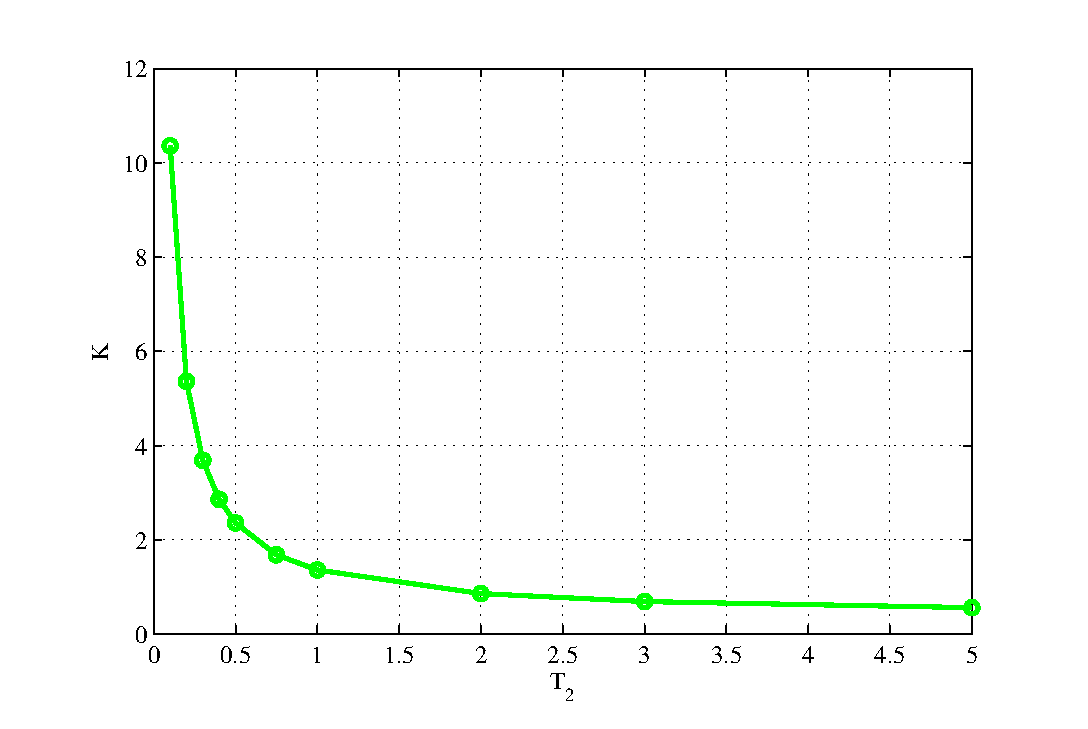
\includegraphics[width=1\linewidth]{scheme/plot4.eps}
	\caption{Теоретическая граница устойчивости на плоскости двух параметров $K, T_2$}
\end{figure}

\newpage
\begin{center}
	\section*{Вывод}
\end{center}
\par
В ходе лабораторной работы был рассмотрен метод управления устойчивостью системы путём изменения отдельных её параметров, таких как  $T_2$ и $K$ при фиксированном значении $T_1$. На основе критерия Гурвица были получены значения для построения графика границы устойчивости аналитическим методом. Аналитически полученные результаты совпадают с полученными в результате математического моделирования. Следовательно, можно сделать вывод, что устойчивость системы определяется не характером возмущения, а структурой самой системы.

\end{document}